%! Author = verwoerd
%! Date = 18-6-2023

% Preamble
\documentclass[11pt,pdf, aspectratio=169]{beamer}
\usetheme{metropolis}

% Packages
\usepackage{amsmath}
\usepackage[utf8]{inputenc}
\usepackage[T1]{fontenc}
\usepackage{graphicx}
\usepackage{tikz}
\usepackage{minted}
\usepackage[
  type={CC},
  modifier={by-sa},
  version={4.0},
]{doclicense}
\setsansfont{Fira Sans}
\usemintedstyle{manni}
\setminted{
  fontsize=\footnotesize,linenos,frame=lines, framesep=2mm
}
\usetikzlibrary{external,arrows,shapes}

\title{DAPC 2023 Training Sessions\\Session 1}
\author{Verwoerd}


% Document
\begin{document}
  \maketitle
  \section{Introduction}
  \begin{frame}{Welcome}
    \begin{itemize}
      \item Welcome to the DAPC 2023 Training Sessions
      \item 4 sessions
      \item We will discuss all last years problems of the DAPC and BAPC
      \item Every session some problems we solve together
      \item Other problems you can solve in between sessions and only the solutions will be presented
      \item Every session starts with some practical information
      \item Maybe guest speakers?
    \end{itemize}
  \end{frame}
  \begin{frame}{Who am I}
    \begin{itemize}
      \item Alumnus, working in the Software Industry
      \item Involved in organizing programming contests since 2003 as volunteer
      \item ``Coach'' for TU Delft teams since NWERC 2003
      \item Twice coach on the World Finals
    \end{itemize}
    \doclicenseThis
  \end{frame}
  \begin{frame}{Session 1 (Today)}
    \begin{itemize}
      \item Introduction to Programming Contests
      \item Reading a problem
      \item Introduction to DOMJudge
      \item Some tips on estimate the problem complexity
      \item Solving an ad-hoc Math problem
      \item Meet and Greet to look for team or team-members
    \end{itemize}
  \end{frame}
  \begin{frame}{Session 2}
    \begin{itemize}
      \item Team Tactics
      \item Utilizing the Test Session
      \item How to select problems
      \item Dealing with wrong submissions
      \item Solutions to the Ad-hoc and Math Problems
      \item Solving Sorting and Search Problems
    \end{itemize}
  \end{frame}
  \begin{frame}{Session 3}
    \begin{itemize}
      \item Creating a team Reference Document
      \item Solutions to Sorting and Search Problems
      \item Solving Interactive Problems and Randomized Input Problems
    \end{itemize}
  \end{frame}
  \begin{frame}{Session 4}
    \begin{itemize}
      \item Role of the coach on big contests
      \item Tips, tricks and common mistakes
      \item Solutions to the Interactive Problems and Randomized Input Problems
      \item Solving the Hardest Problems
    \end{itemize}
  \end{frame}
  \section{Introduction to Programming Contests}
  \begin{frame}{What is a programming contest?}
    \begin{itemize}
      \item<1-> Team of 3 people
      \item<1-> Single computer
      \item<1-> Solve as many problems from the problem set (8 to 15 problems)
      \item<1-> In any order
      \begin{itemize}
        \item<2-> Solve it efficiently
        \item<2-> do it as quickly as possible (under pressure)
        \item<2-> and do it correctly (without bugs)
      \end{itemize}
      \item<1-> In 5 hours
      \item <3-> With limited documentation and no internet
    \end{itemize}
  \end{frame}
  \begin{frame}{How is score calculated?}
    \begin{itemize}
      \item<1-> Sorted by number of problems solved
      \item<2-> Sorted by the total time for solved problems
      \begin{itemize}
        \item<3->  Time in minutes since the start of the contest
        \item<3-> Penalty for each wrong attempt on a solved solution of 20 minutes
        \begin{itemize}
          \item<4-> Penalty time is counts only if the problem is solved afterward.
          \item<4-> Penalty time does not reduce your contest time.
          \item<4-> Penalty time is not added after wrong attempts after the problem is solved.
          \item<4-> No penalty for compiler errors.
        \end{itemize}
      \end{itemize}
    \end{itemize}
  \end{frame}
  {
    \setbeamertemplate{background canvas}{
      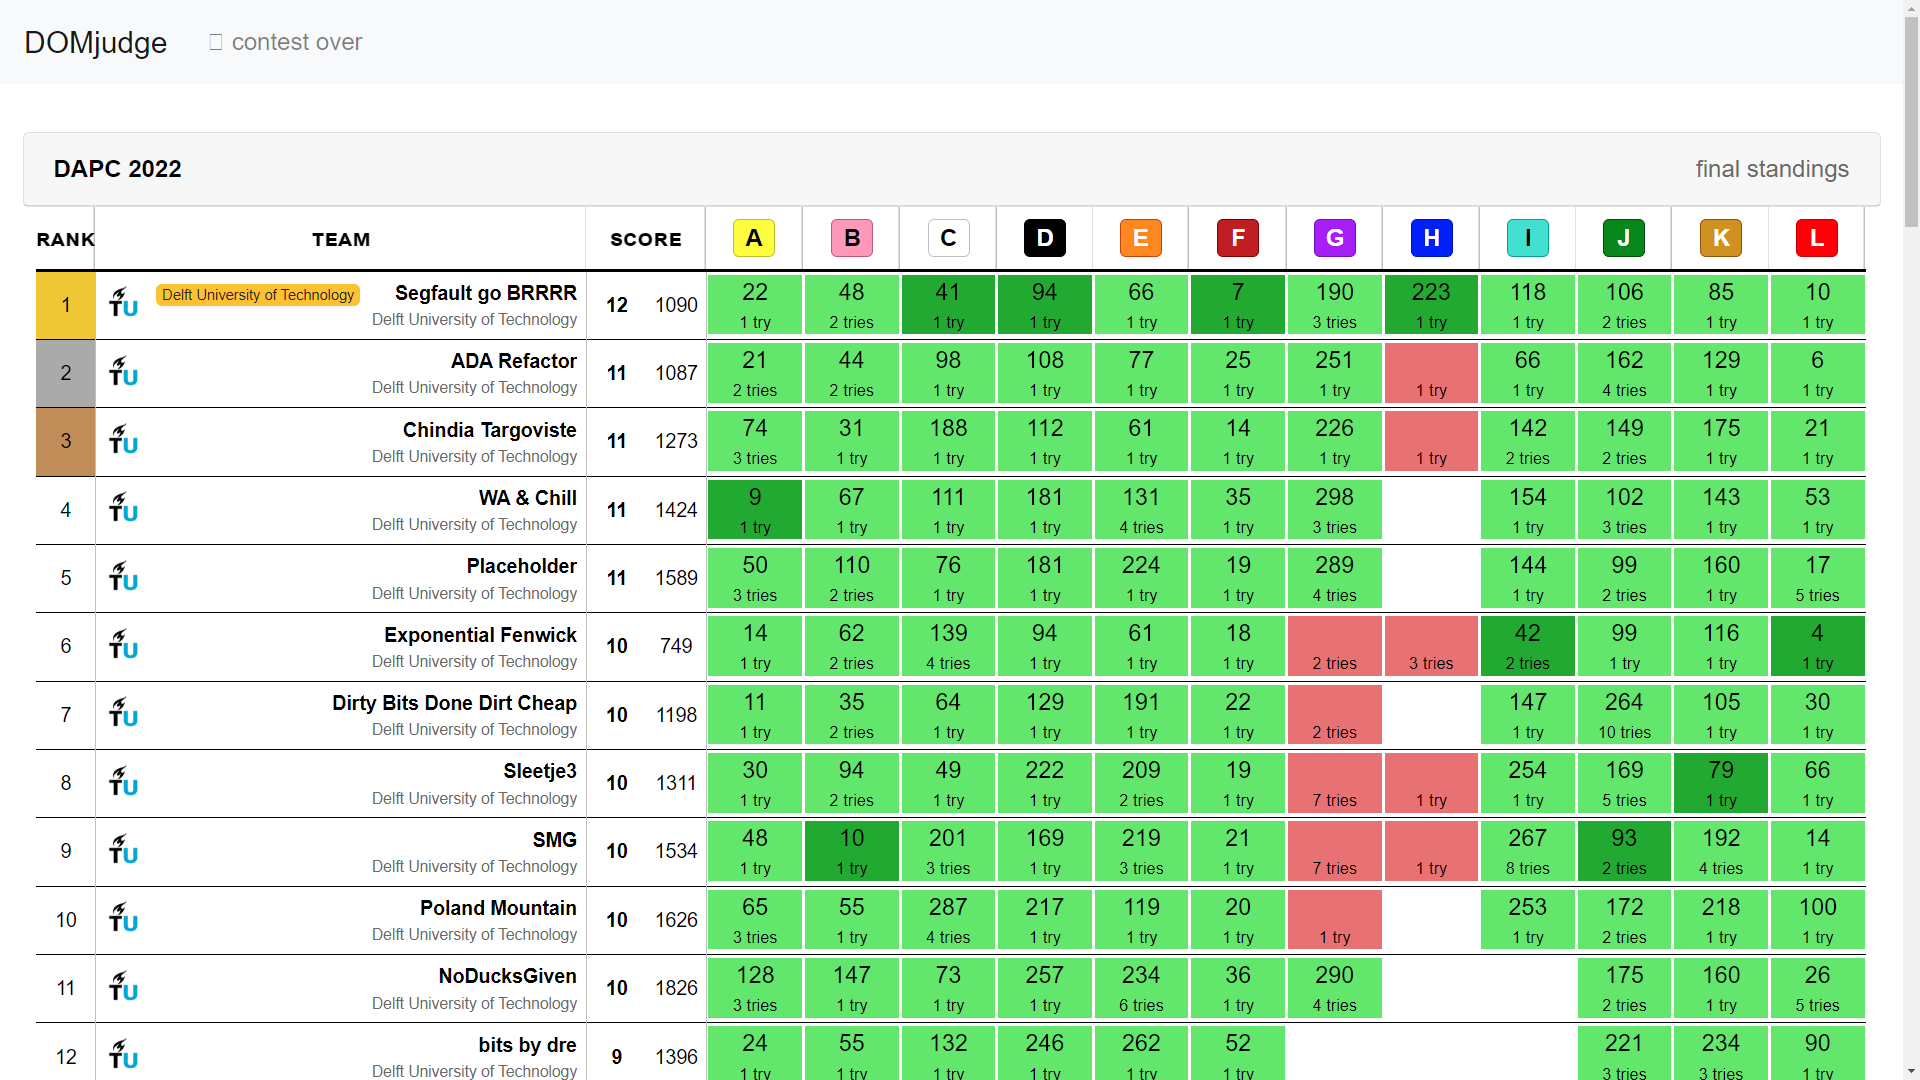
\includegraphics[height=\paperheight]{images/session-1/scoreboard}
    }
    \begin{frame}{Example Scoreboard}
    \end{frame}
  }
  \begin{frame}{Road to the world finals}
    The DAPC is an official preliminary of the ICPC.
    \begin{tikzpicture}
  \tikzstyle{every node}=[draw]
  \node {International Collegiate Programming Contest World Finals}
    child {node[red]{NWERC}
        child { node[red] {BAPC}
          child {node[red] {DAPC} edge from parent node[left, draw=none]{\textasciitilde 5 best teams}}
          child {node {AAPP}}
          child {node {EAPC}}
          child {node {TAPC}}
          child {node {$\ldots$}}
          edge from parent node[left, draw=none]{\textasciitilde3 best teams per university}
        }
    child {node{GCPC}}
    child {node{NCPC}}
    child {node{UKIEPC}}
    edge from parent node[left, draw=none] {\textasciitilde3 best teams}
  }
  child {node {NAC}}
  child {node{SWERC}}
  child {node{$\ldots$}};

\end{tikzpicture}

  \end{frame}
  \section{Reading a problem}
  \begin{frame}{Problem structure}
    A typical problem has the following structure
    \begin{itemize}
      \item Problem description
      \item Input description
      \item Output description
      \item Example input/output
      \item A time limit in seconds
    \end{itemize}
    You are asked to write a program that solves the problem for all valid inputs within the time limit.
  \end{frame}
  \begin{frame}{Example problem}
    \begin{block}{Problem description}
      Write a program that multiplies pairs of integers
    \end{block}
    \vspace{10pt}
    \begin{block}{Input description}
      Input starts with one line containing an integer $T$, where $1\leq T \leq 100$, denoting the number of test cases.
      Then $T$ lines follow, each containing a test case.
      Each test case consists of two integers $A,B$, where $-10^{6} \leq A,B \leq 10^{6}$, separated by a single space.
    \end{block}

    \vspace{10pt}

    \begin{block}{Output description}
      For each test case, output one line containing the value of $A\times B$.
    \end{block}
  \end{frame}
  \begin{frame}{Example problem}
    \begin{center}
      \begin{tabular}{|l|l|}
        \hline
        {\footnotesize Sample input} & {\footnotesize Sample output} \\
        \hline
        \begin{minipage}{80pt}
          \vspace{10pt}
          \ttfamily
          4\\
          3 4\\
          13 0\\
          1 8\\
          100 100\\
        \end{minipage}
        &
        \begin{minipage}{80pt}
          \vspace{10pt}
          \ttfamily
          12\\
          0\\
          8\\
          10000\\
        \end{minipage}
        \\
        \hline
      \end{tabular}
    \end{center}
  \end{frame}
  \begin{frame}[containsverbatim]{Solution in c++}
    \inputminted{c++}{code/session-1/c++/example-wrong.cpp}
  \end{frame}
  \begin{frame}[containsverbatim]{Solution in java}
    \inputminted{java}{code/session-1/java/example-wrong.java}
  \end{frame}
  \begin{frame}[containsverbatim]{Solution in kotlin and Python}
    \inputminted{kotlin}{code/session-1/kotlin/example-wrong.kt}
    \inputminted{python}{code/session-1/python/example.py}
  \end{frame}
  \section{Introduction to DOMJudge}
  \begin{frame}{Submitting the Solution}
    \begin{itemize}
      \item During the contest you submit to a contest control system
      \begin{itemize}
        \item Usually DOMJudge, but sometimes Kattis or PC\^ 2
      \end{itemize}
      \item Submit solutions
      \item Ask questions about the problems or programming environment
      \item Read clarifications from the jury
    \end{itemize}
  \end{frame}
  \begin{frame}{Domjudge Interface - home}
    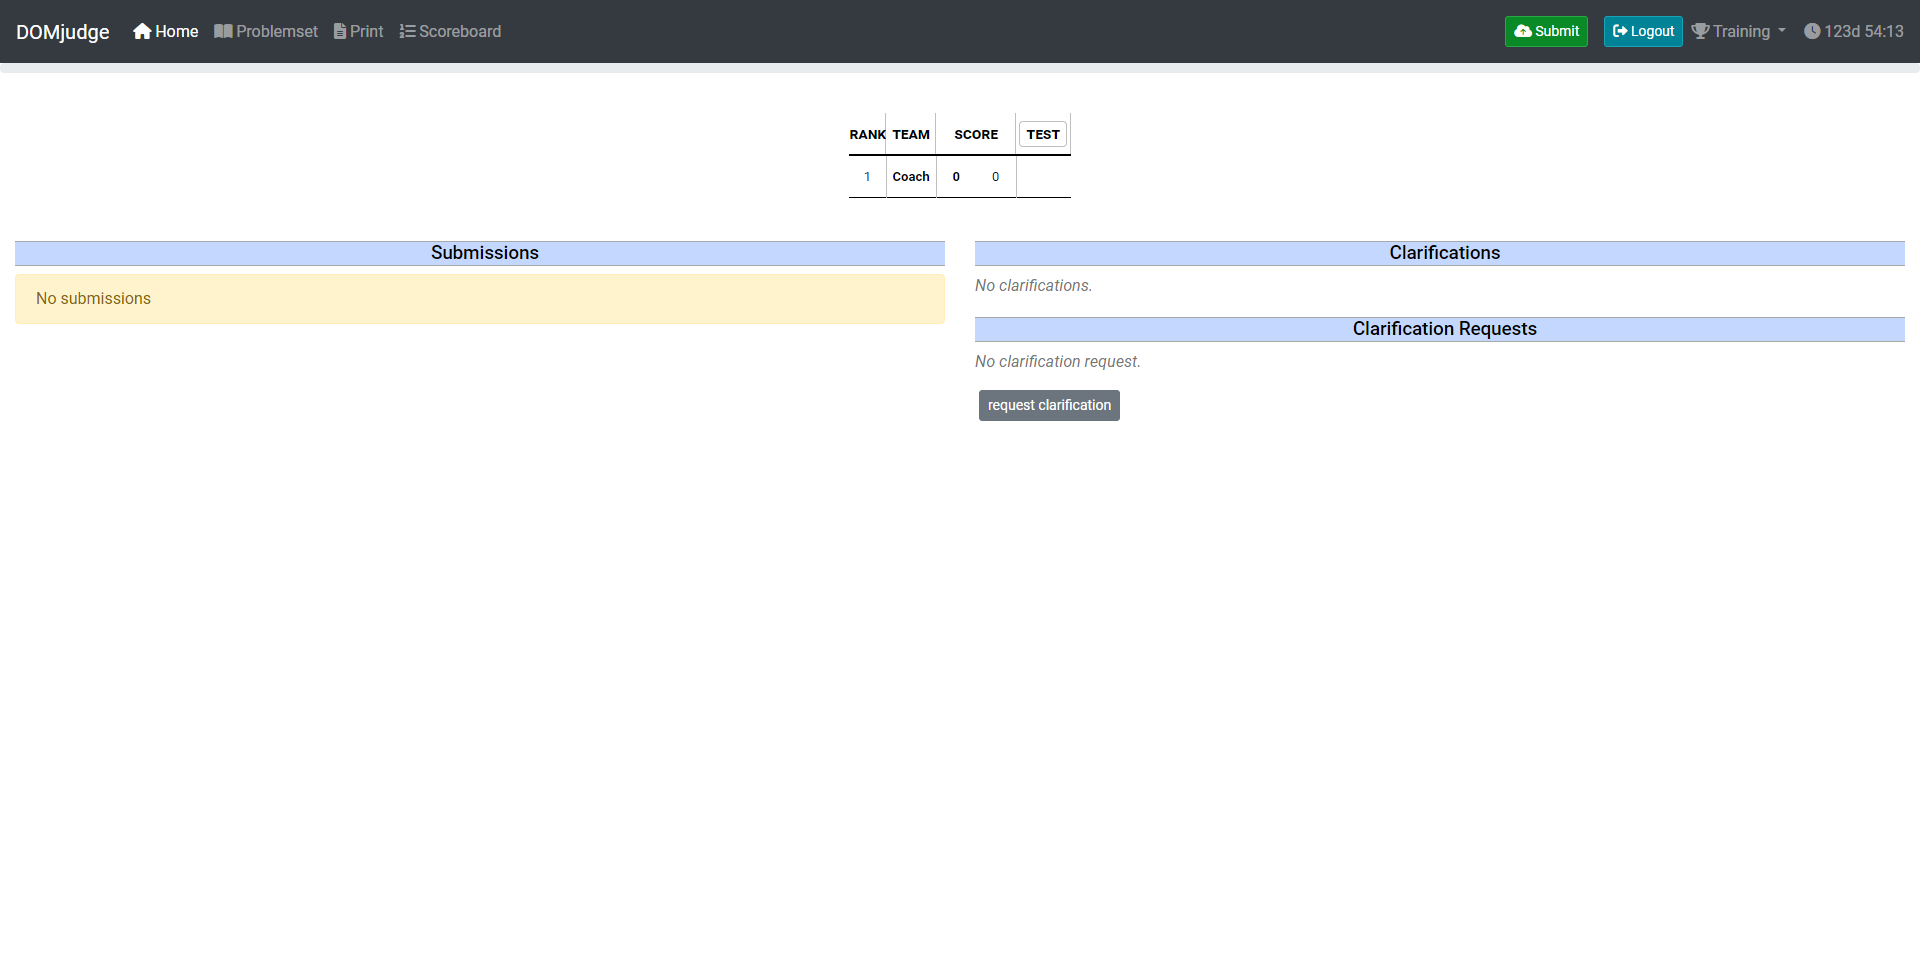
\includegraphics[width=\linewidth]{images/session-1/domjudge-initial}
  \end{frame}
  \begin{frame}{Domjudge Interface - problems}
    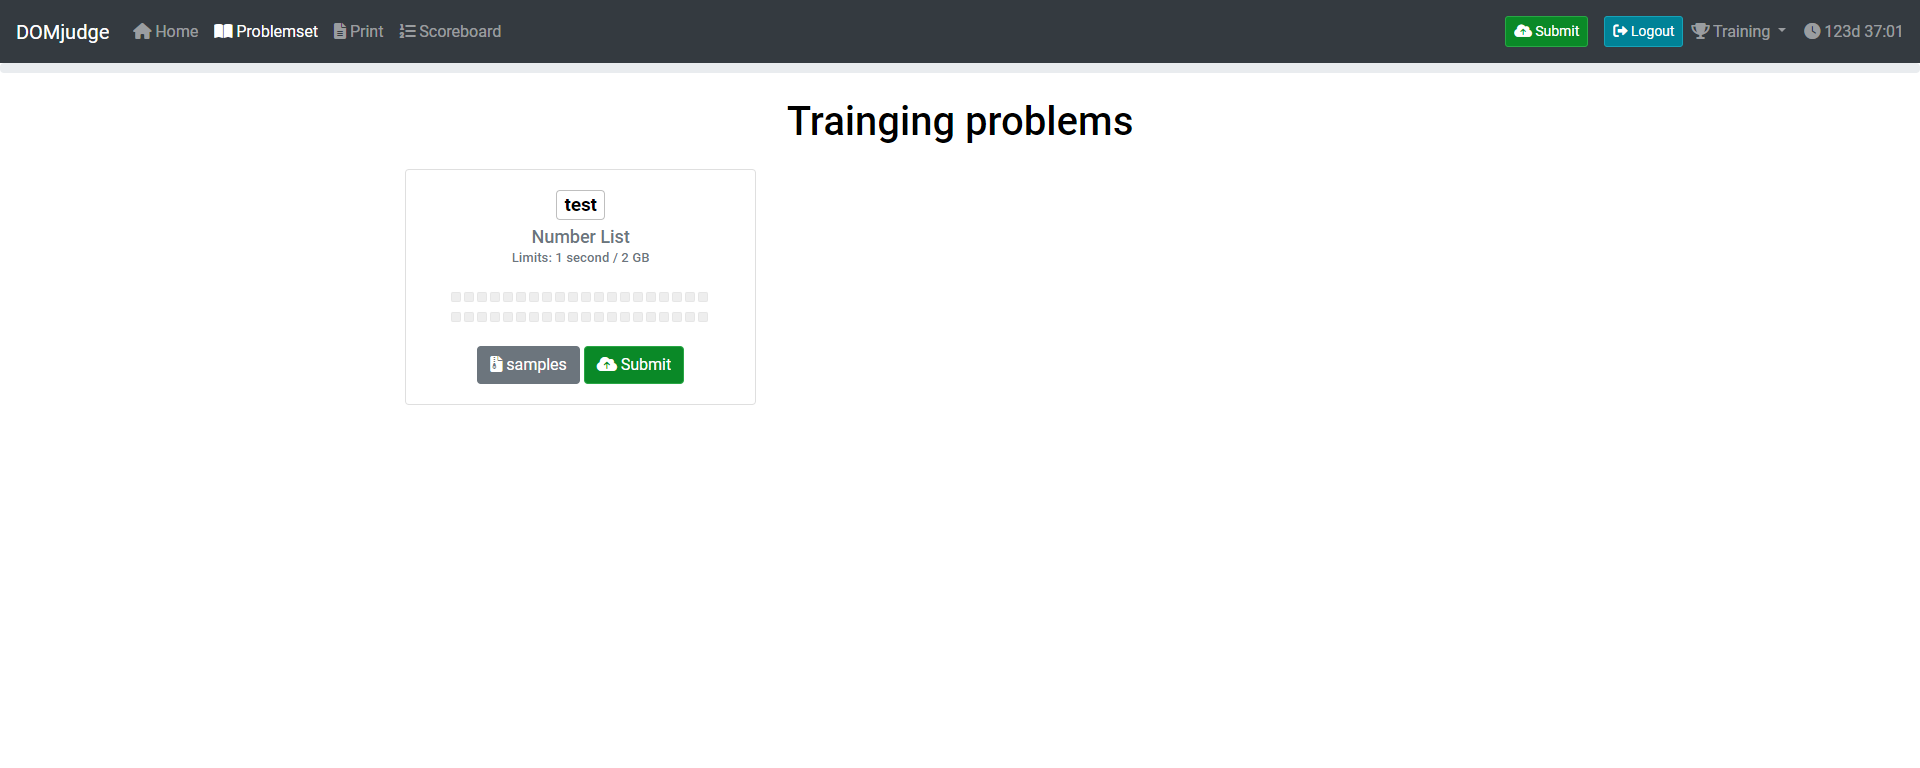
\includegraphics[width=\linewidth]{images/session-1/domjudge-problems}
  \end{frame}
  \begin{frame}{Domjudge Interface - submit}
    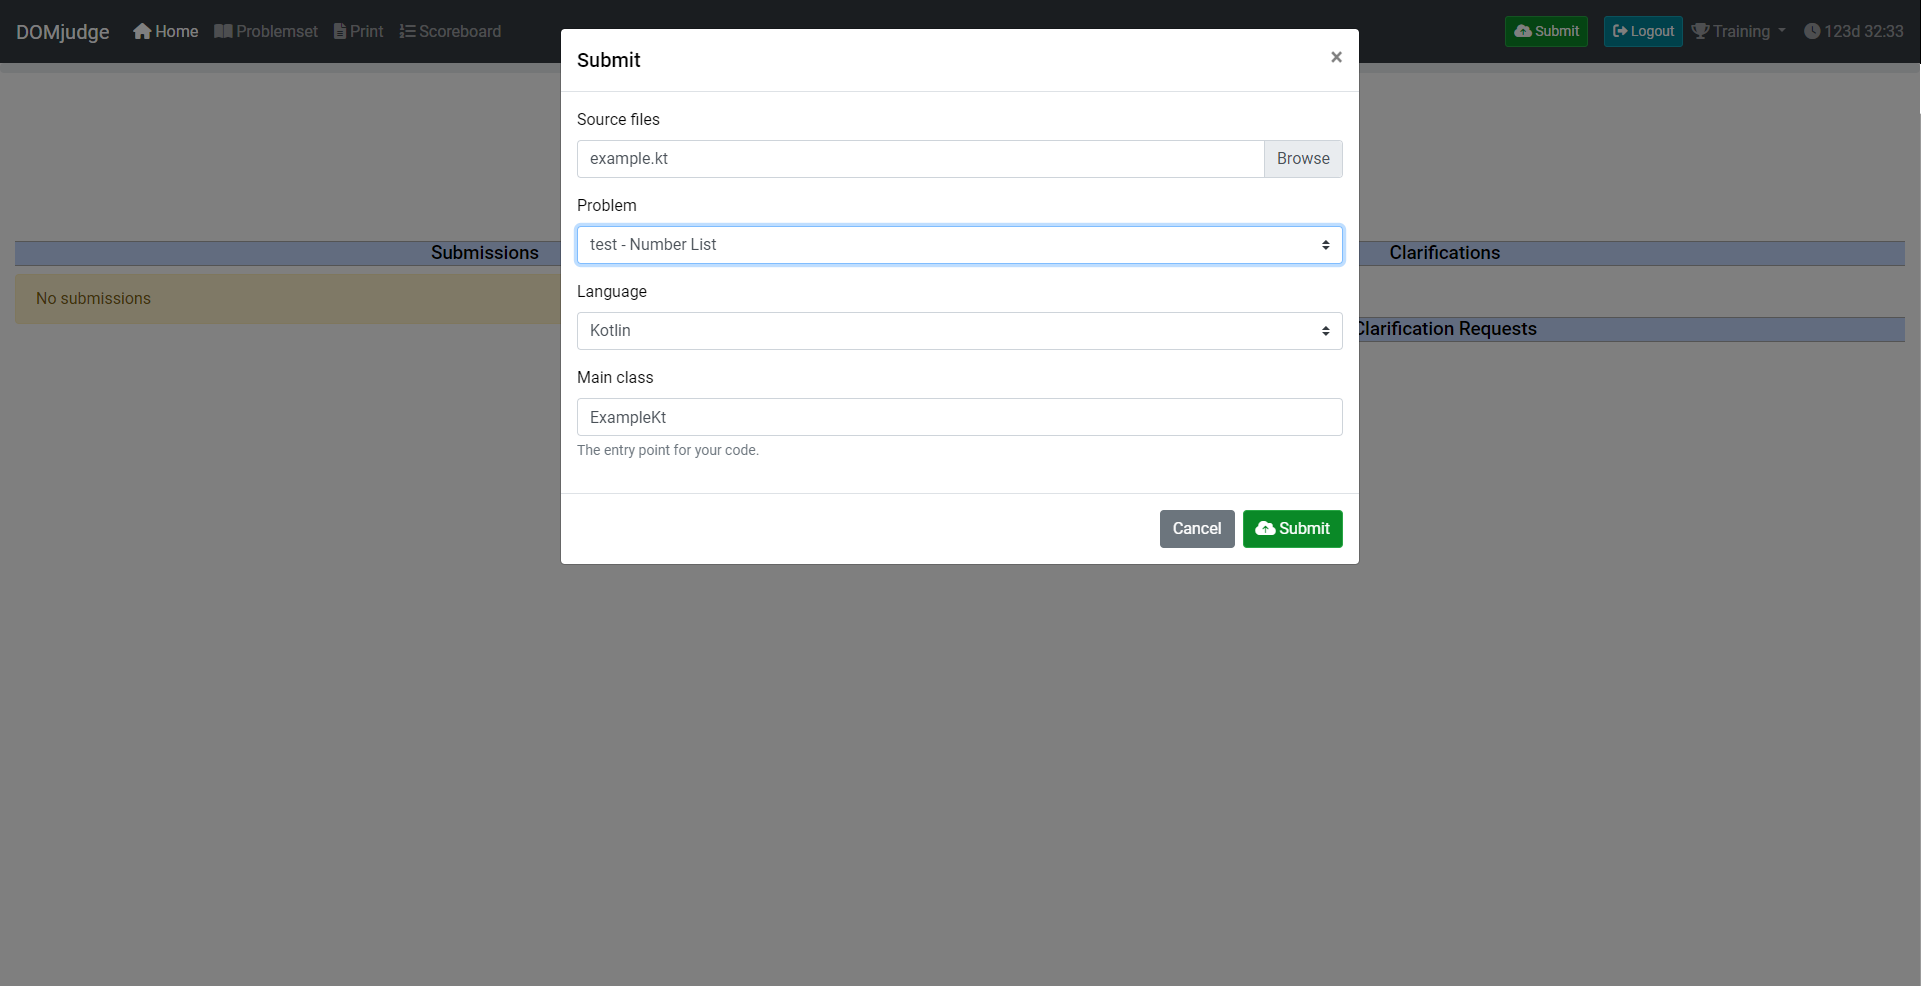
\includegraphics[width=\linewidth]{images/session-1/domjudge-submit}
  \end{frame}
  \begin{frame}{Are the solutions correct?}
    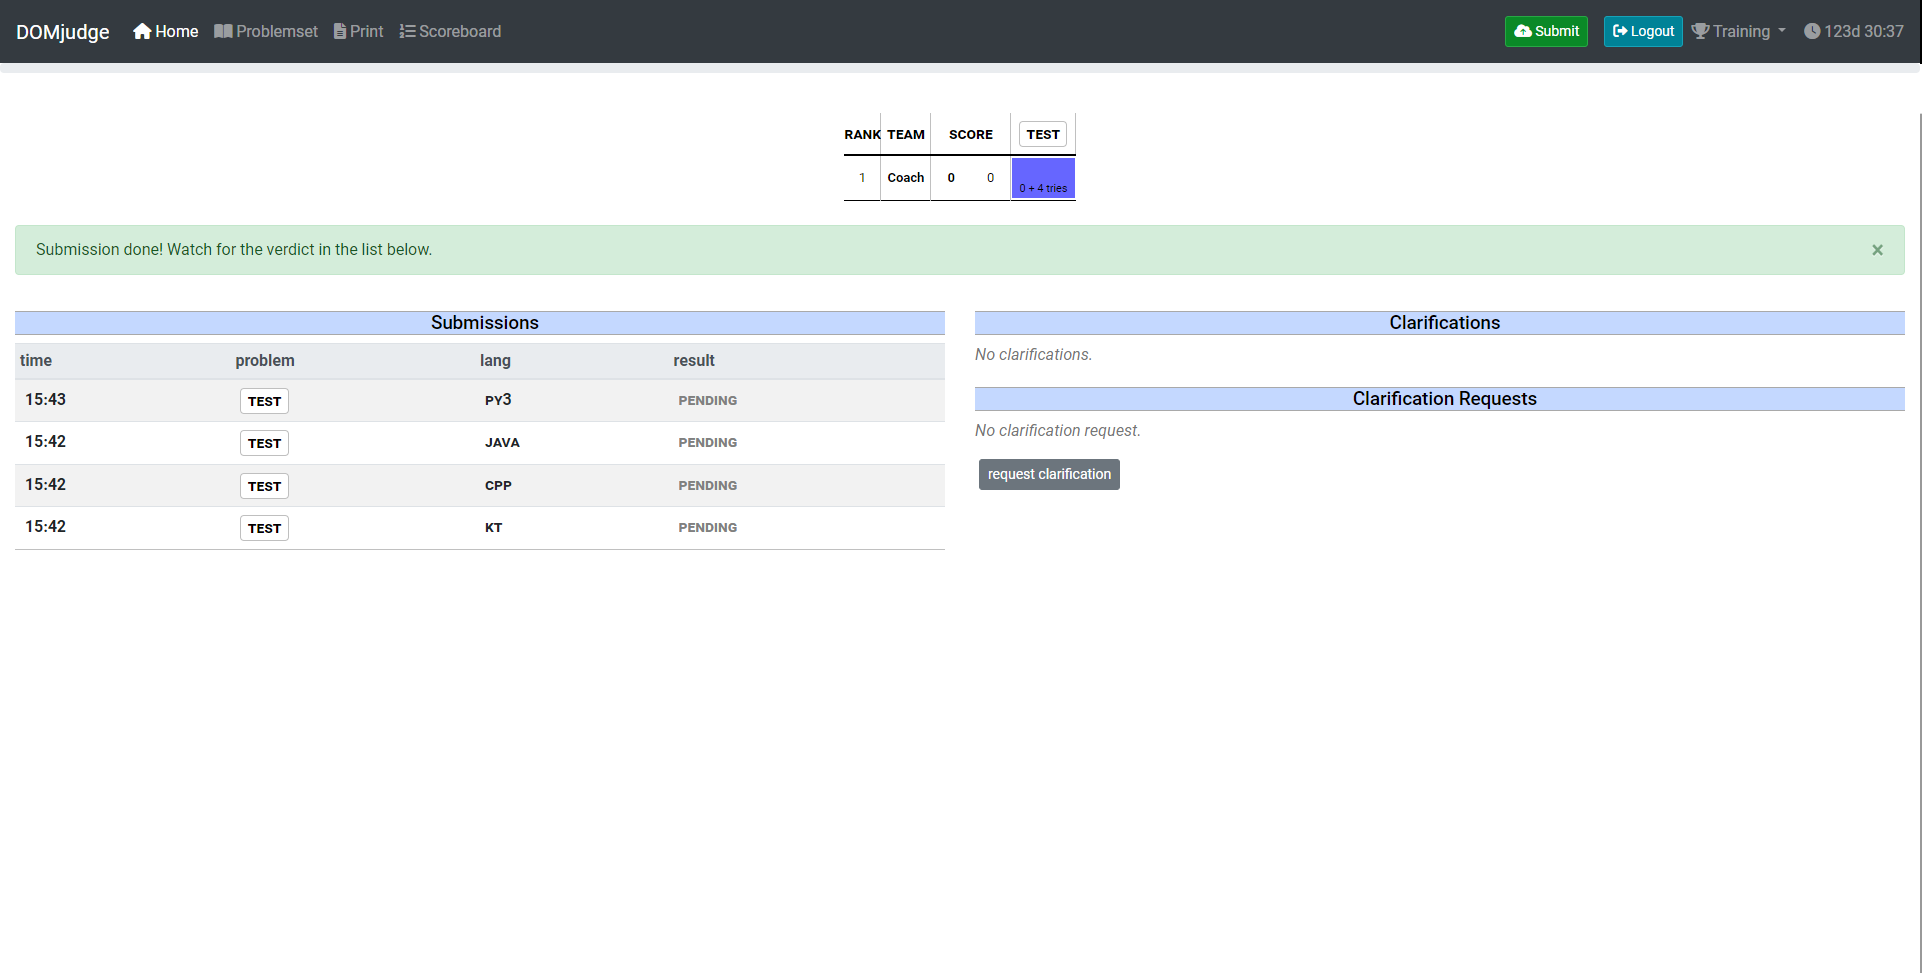
\includegraphics[width=\linewidth]{images/session-1/domjudge-submit-first-try}
  \end{frame}
  \begin{frame}{We made a whoopsy?}
    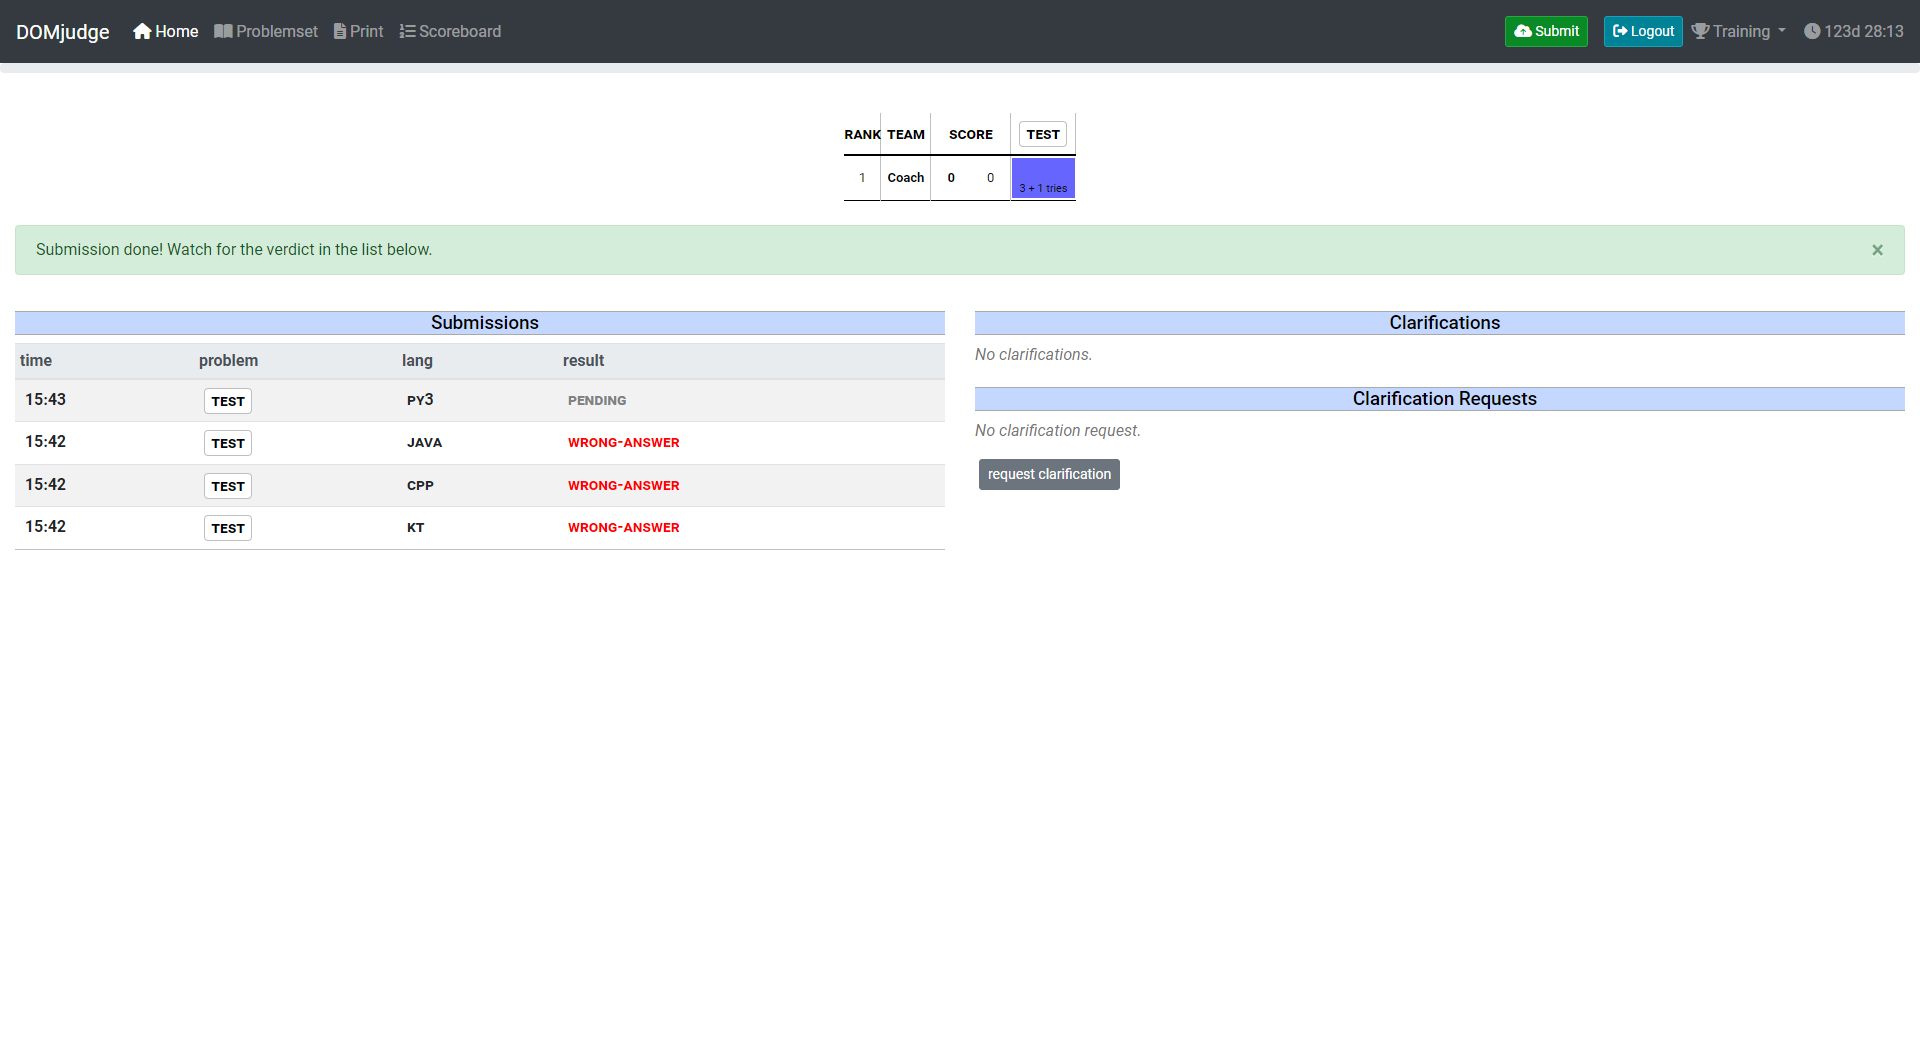
\includegraphics[width=\linewidth]{images/session-1/domjudge-no-double}
  \end{frame}
  \begin{frame}{Or not}
    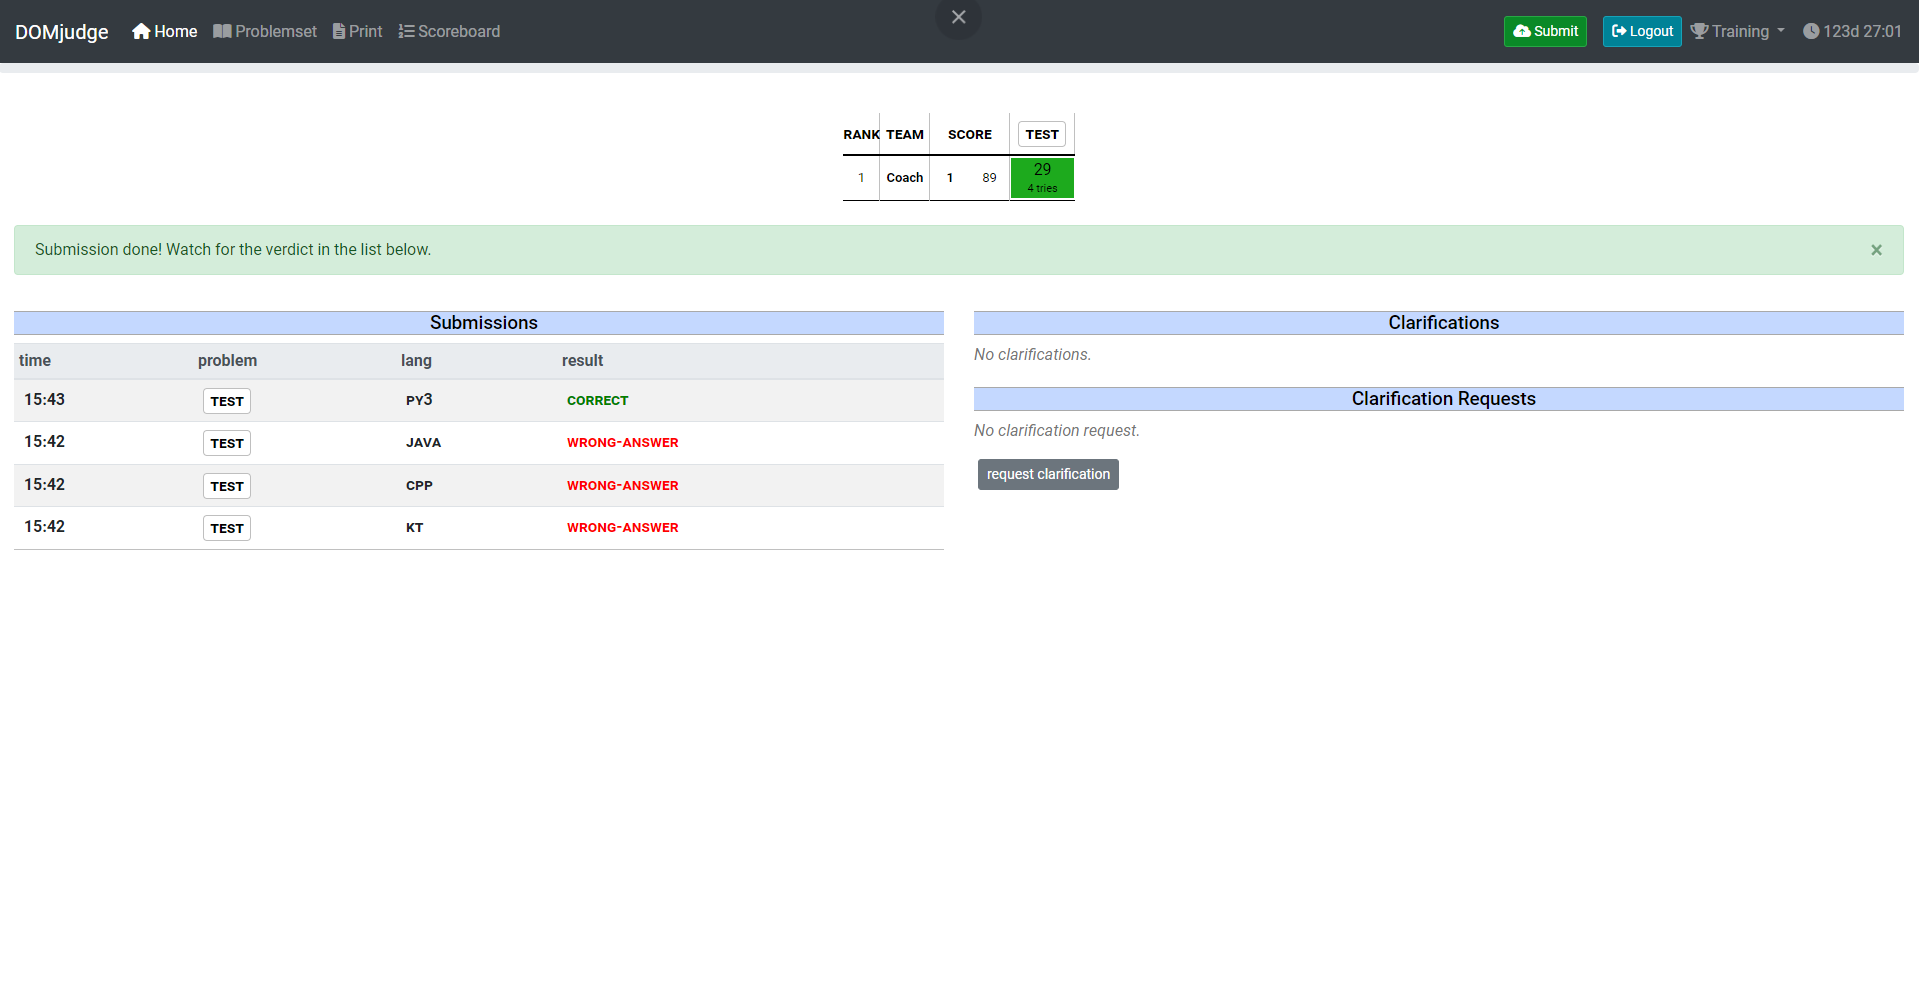
\includegraphics[width=\linewidth]{images/session-1/domjudge-correct}
  \end{frame}
  \begin{frame}{Lets ask the jury}
    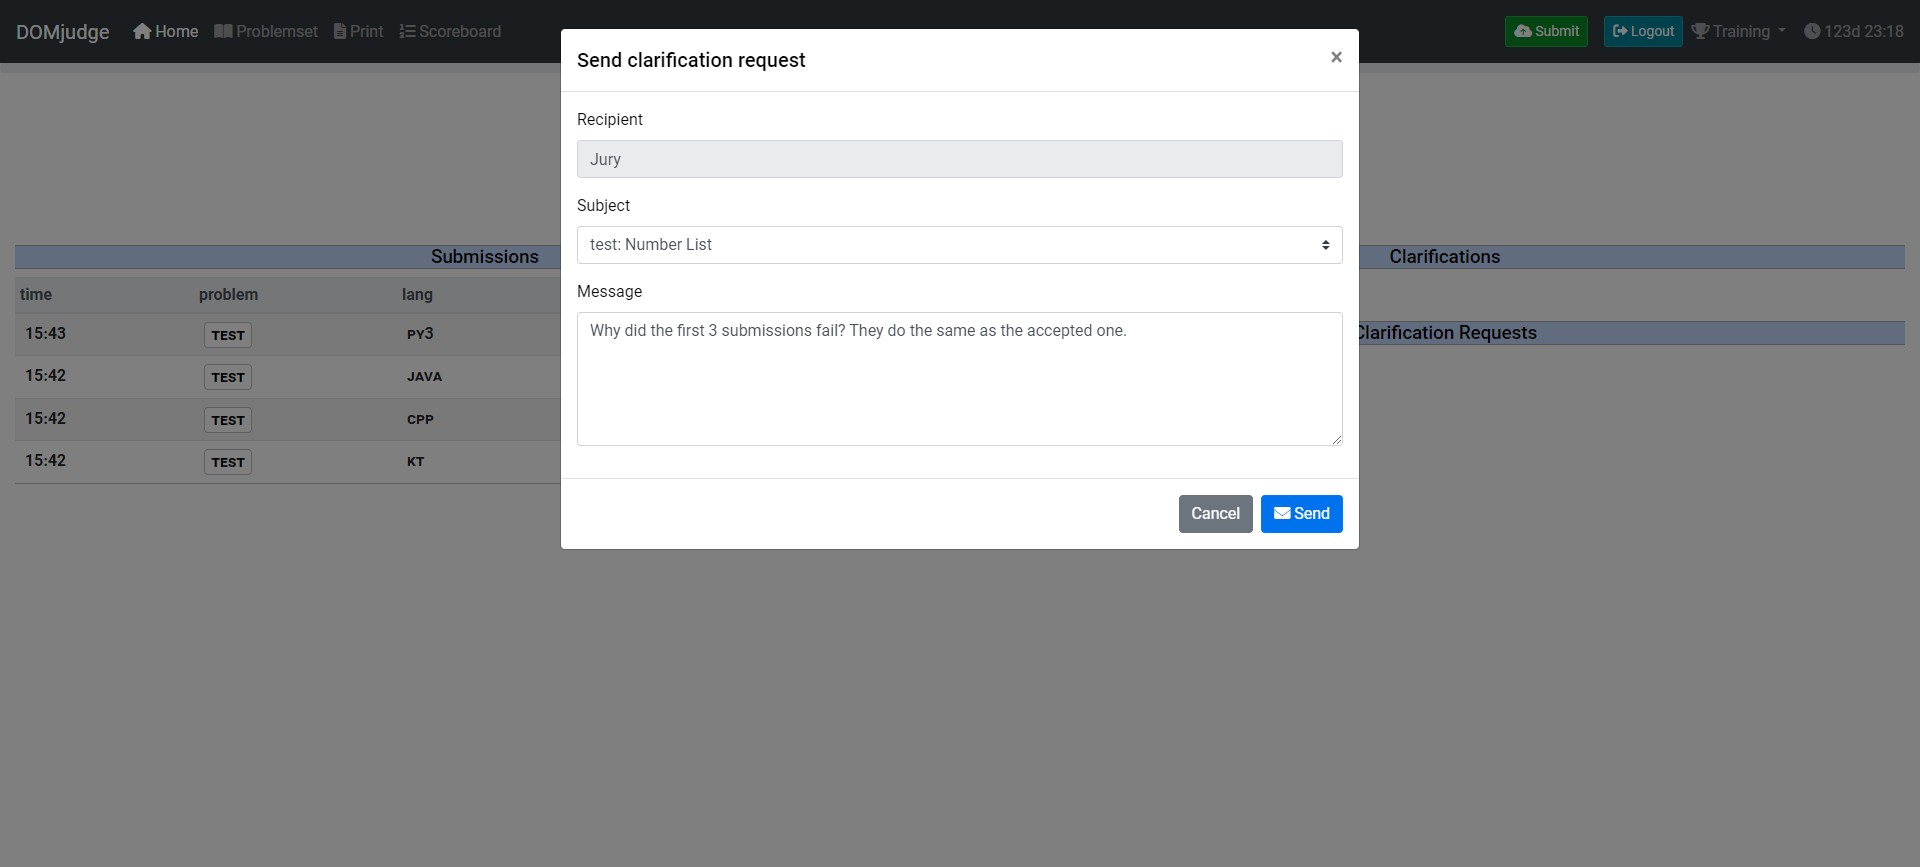
\includegraphics[width=\linewidth]{images/session-1/domjudge-clar-1}
  \end{frame}
  \begin{frame}{Lets hope they respond fast}
    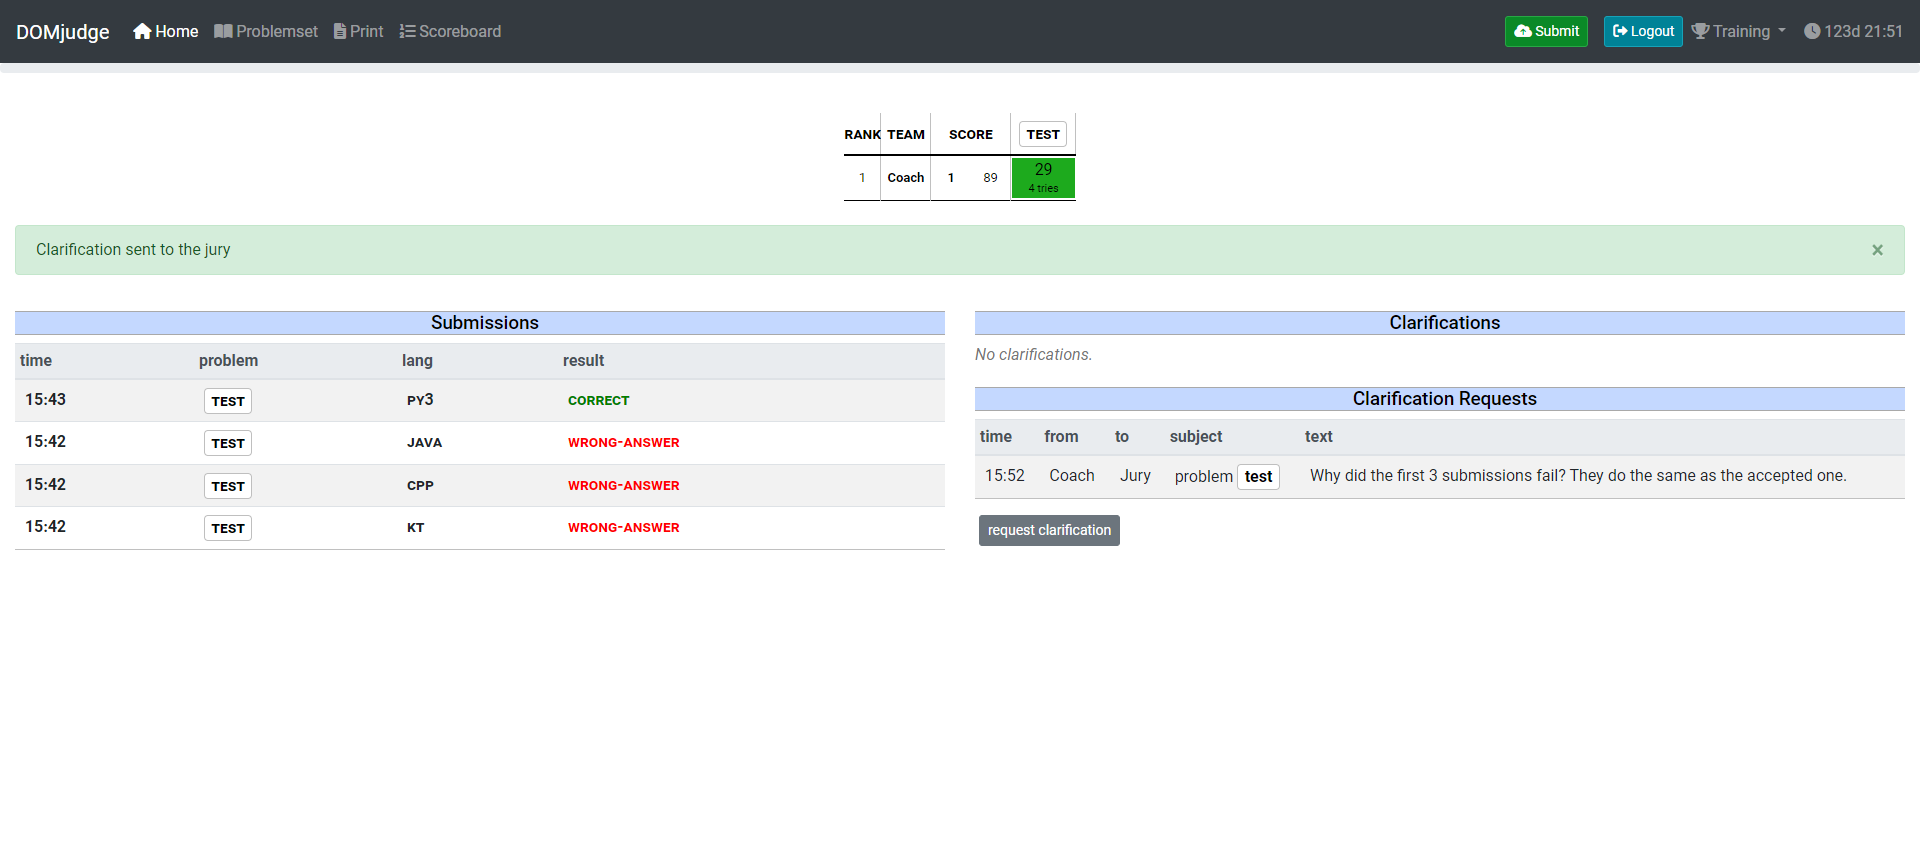
\includegraphics[width=\linewidth]{images/session-1/domjudge-clar-2}
  \end{frame}
  \begin{frame}{We have a response}
    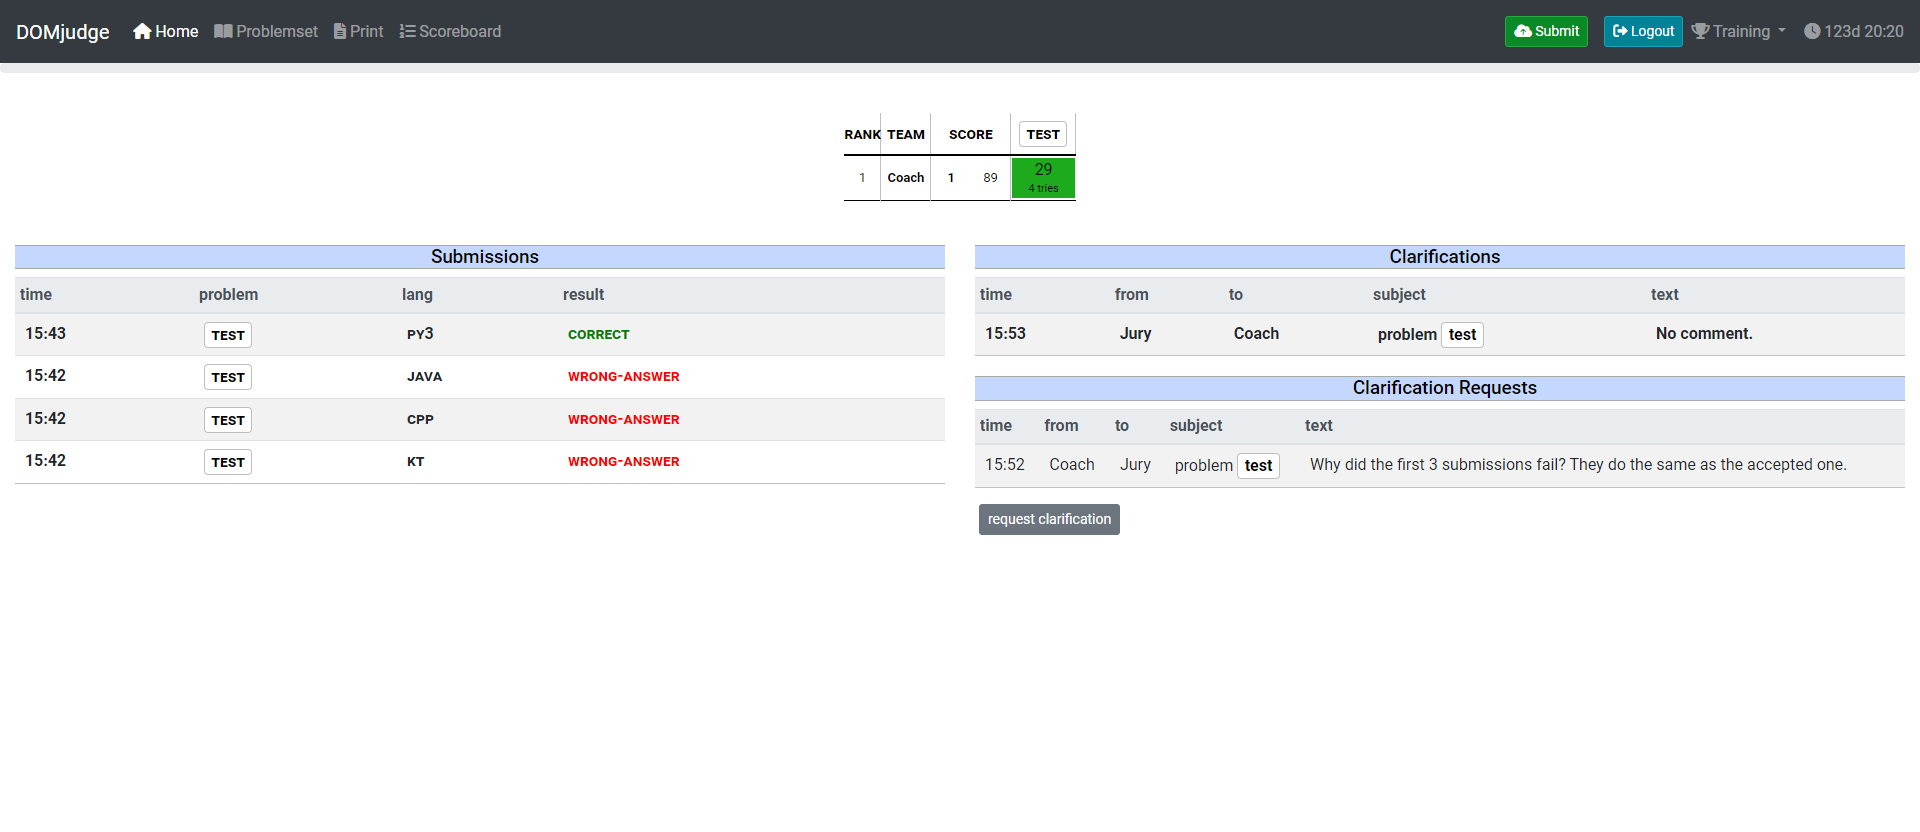
\includegraphics[width=\linewidth]{images/session-1/domjudge-clar-3}
  \end{frame}
  \begin{frame}{The jury is not helping us}
    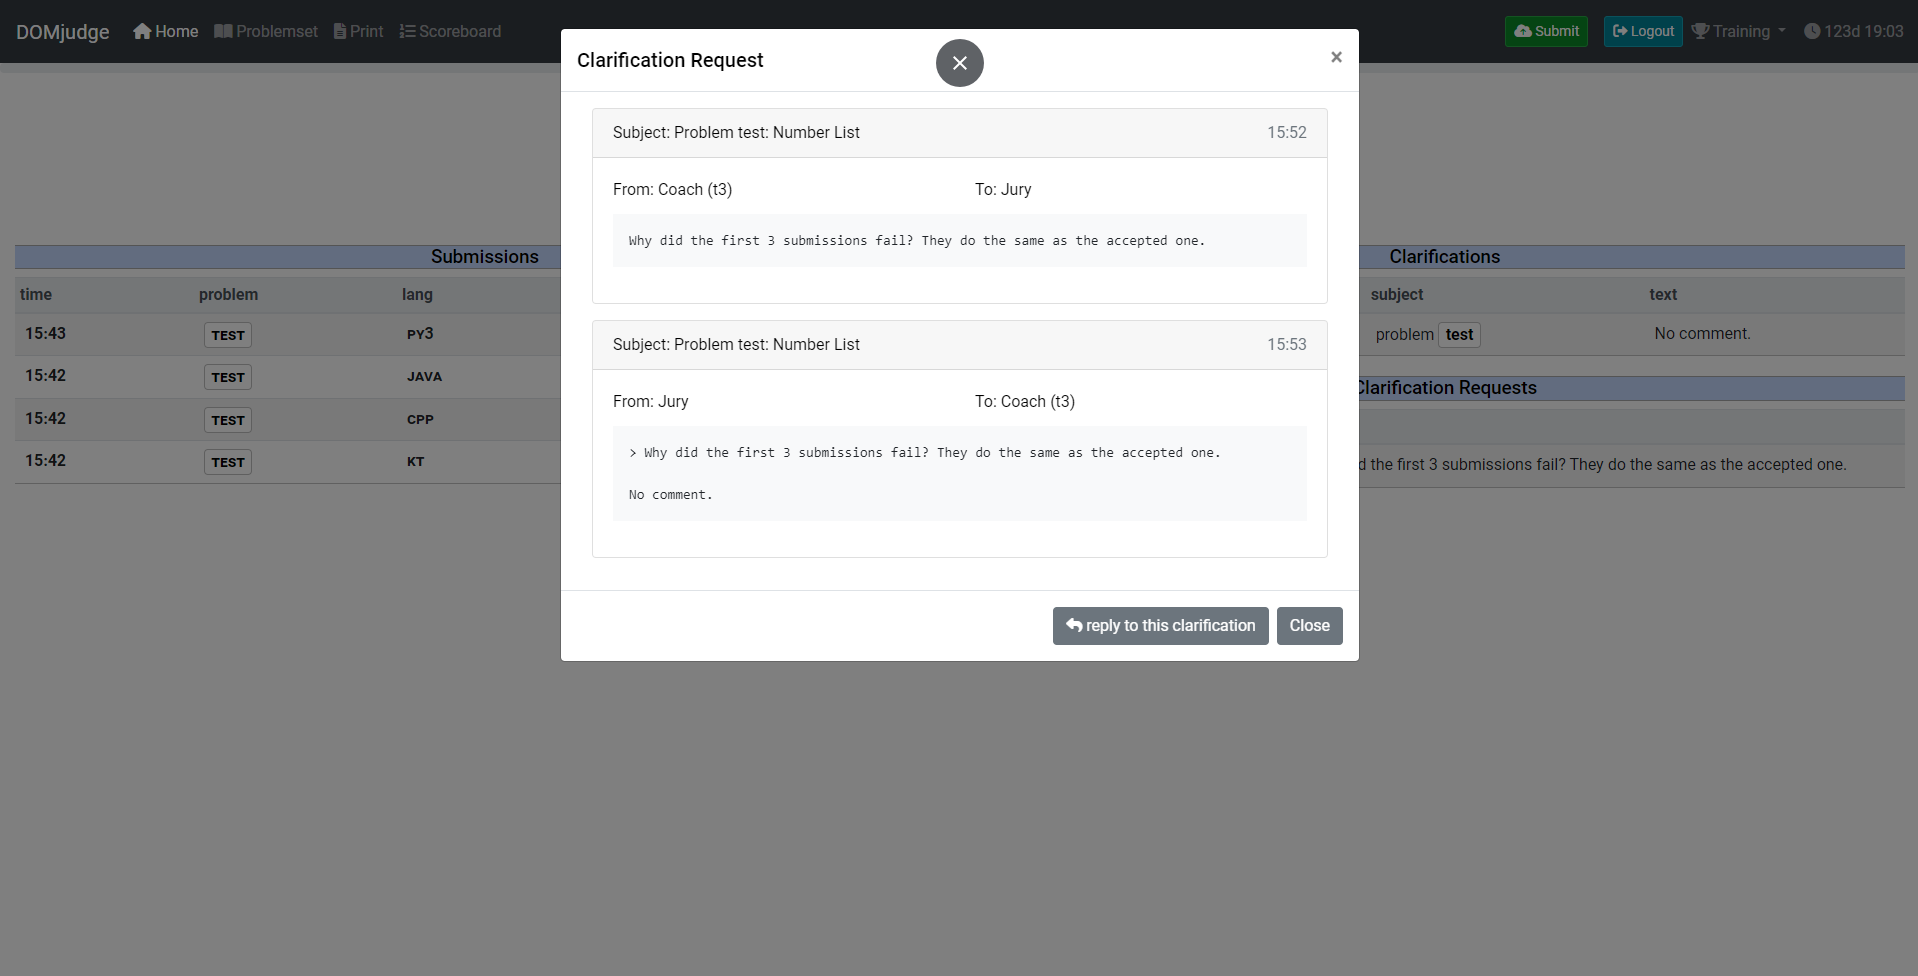
\includegraphics[width=\linewidth]{images/session-1/domjudge-clar-4}
  \end{frame}
  \begin{frame}{Why did the 3 solutions fail?}
    \begin{itemize}
      \item <1-> Lets check the input again: $-10^{6} \leq A,B \leq 10^{6}$
      \item <2-> Worst case scenario: $A=10^6$ and $B=10^6$ giving  $A \times B = 10^{12}$
      \item <3-> Does $10^{12}$ fit in a 32-bit \texttt{int}?
      \item <4-> $\log_2 10^{12} \approx 40$, so \textbf{NO}, 40 bits don't fit in an \texttt{int}
      \item <5-> Use \texttt{long (long)} when possible, except in Python
    \end{itemize}
  \end{frame}
  \begin{frame}[containsverbatim]{Solution in c++}
    \inputminted{c++}{code/session-1/c++/example.cpp}
  \end{frame}
  \begin{frame}[containsverbatim]{Solution in java}
    \inputminted{java}{code/session-1/java/example.java}
  \end{frame}
  \begin{frame}[containsverbatim]{Solution in kotlin}
    \inputminted{kotlin}{code/session-1/kotlin/example.kt}
  \end{frame}
  \begin{frame}{All solutions correct}
    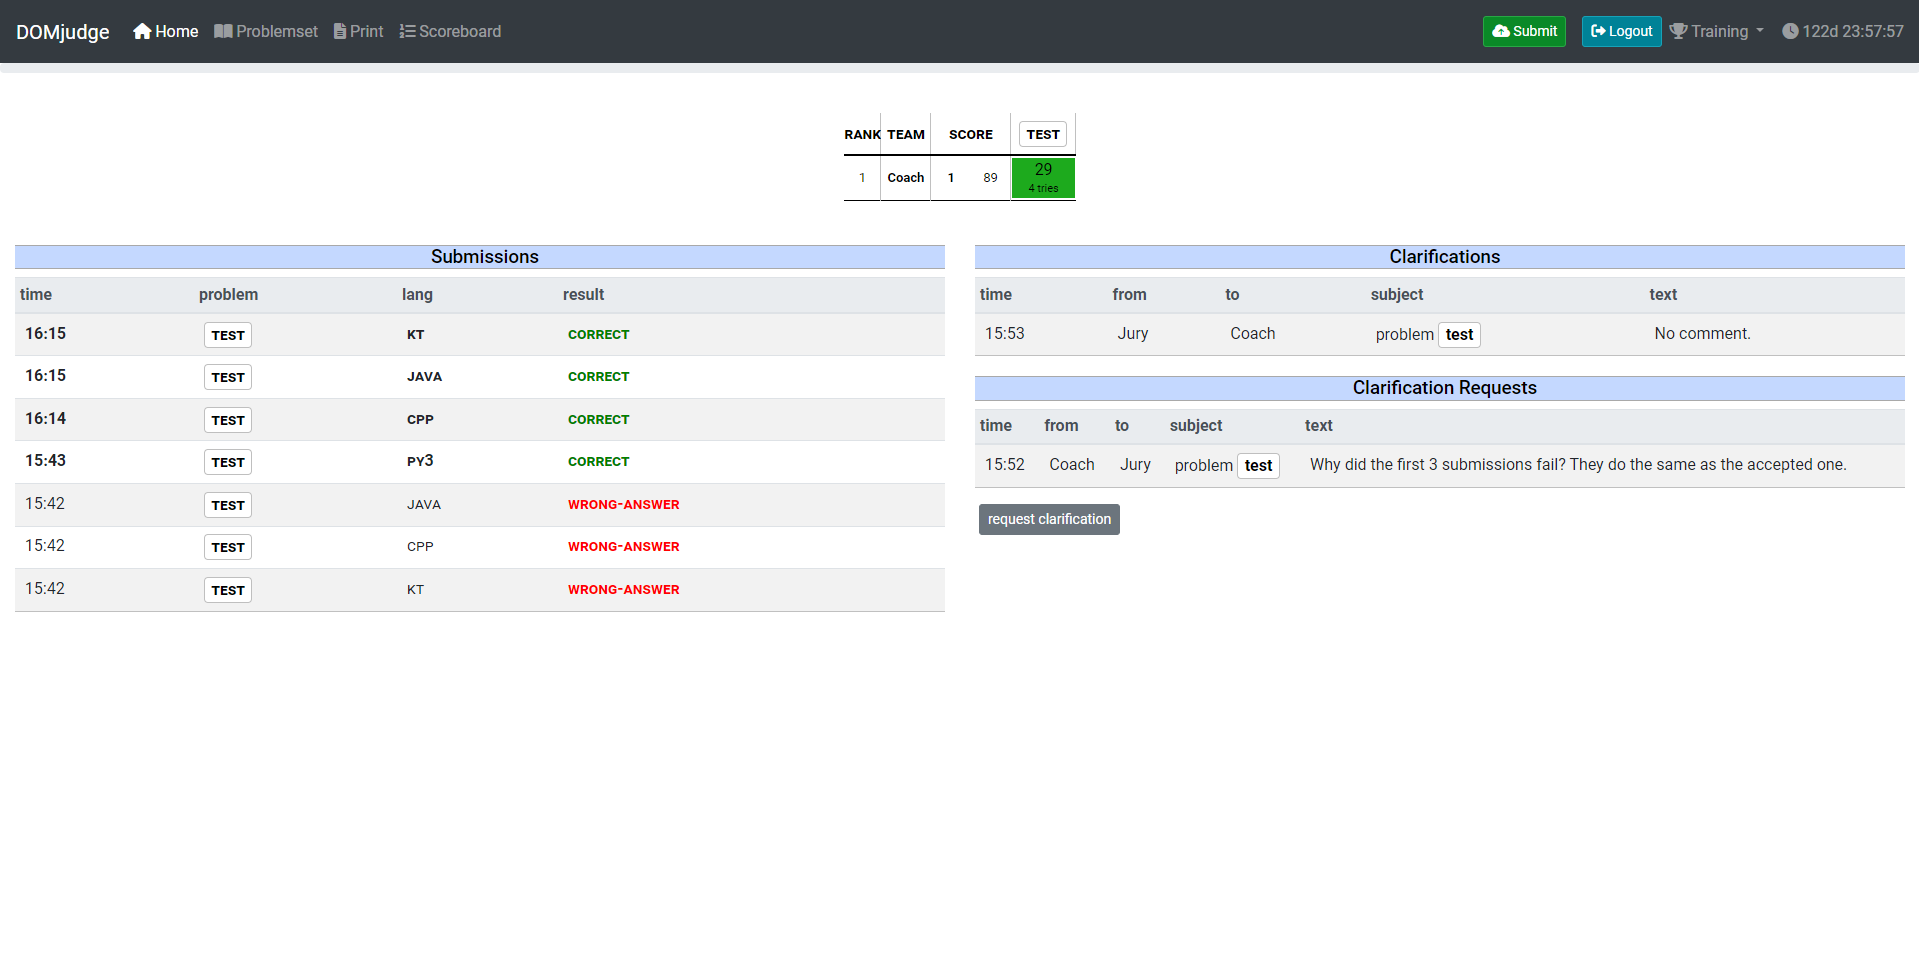
\includegraphics[width=\linewidth]{images/session-1/domjudge-all-correct}
  \end{frame}
  \section{Estimating problem complexity}
  \begin{frame}{About time limit}
    \begin{itemize}
      \item The time limit specifies the time you program may run
      \item This includes JVM-startup and I/O
      \item High time limit signify \begin{itemize}
                                      \item lots of I/O
                                      \item Slower algorithms can be accepted
      \end{itemize}
      \item Low limit signifies fast algorithms, usually the use of formulas
      \item You can use the time limit to check your code on your local machine\\ \texttt{\$ time myjava ProblemA}
    \end{itemize}
  \end{frame}
  \begin{frame}{About input size\footnote[1]{https://gcpc.nwerc.eu/primer.pdf}}
    Based on the input size you can an idea of the time complexity.

    \begin{center}
      \begin{tabular}{llll}
        \hline
        $\mathcal{O}(n!)$         & $n \leq 10$   & $\mathcal{O}(n\log{}^{2}n)$ & $n \leq 10^5$    \\
        $\mathcal{O}(2^n)$        & $n \leq 20$   & $\mathcal{O}(n\log{}n)$     & $n \leq 10^6$    \\
        $\mathcal{O}(n^3)$        & $n \leq 500$  & $\mathcal{O}(n)$            & $n \leq 10^8$    \\
        $\mathcal{O}(n^2\log{}n)$ & $n \leq 1000$ & $\mathcal{O}(\sqrt{n})$     & $n \leq 10^{15}$ \\
        $\mathcal{O}(n^2)$        & $n \leq 5000$ & $\mathcal{O}(\log{}n)$      & $n \leq 10^{18}$ \\
        $\mathcal{O}(n\sqrt {n})$ & $n \leq 10^5$ &                             &                  \\
        \hline
      \end{tabular}
    \end{center}

    \textbf{Warning}: This is not guaranteed to be always the case!
  \end{frame}

  \section{Solving an ad-hoc math problem}
  \begin{frame}{An other problem}
    \begin{itemize}
      \item Source BAPC Preliminaries 2022
      \item Problem name: Fastest Function
      \item Time limit: 1s
    \end{itemize}
    Original problem written by the BAPC 2022 jury and licensed under \doclicenseLongNameRef.

    \doclicenseImage

  \end{frame}
  \begin{frame}{Problem: Fastest Function}
    You are working as a software developer for the Bug Acquisition Programming Company.
    They developed a specific piece of software called Program C that they sell to their clients.
    For the past weeks, you have been working on optimising a specific function \texttt{foo} in the main code path in Program C.
    You have made it a lot faster and would like to show off to your boss about it.

    Your IDE has a nice tool that allows you to profile your code and tell you what percentage of the total running time \texttt{foo} takes.
    You can run this on the version before your change and after your change.
    However, you think it looks a lot cooler if you can just tell your boss how much faster you have made        \texttt{foo} itself.
  \end{frame}
  \begin{frame}{Problem: Fastest Function: Input and Output}
    \textbf{Input}

    The input consists of:
    \begin{itemize}
      \item One line with two integers $x$ and $y$ ($0 < x, y < 100$),
      where $x$ is the percentage of the total running time that \texttt{foo} took before optimising
      and $y$ the percentage of the total running time it took after optimising.
    \end{itemize}

    \textbf{Output}

    Output the factor of how much faster \texttt{foo} got after your optimization.

    Your answer should have an absolute or relative error of at most $10^{-6}$.
  \end{frame}
  \begin{frame}{Problem: Fastest Function: Samples}
    \begin{tabular}{|l|l|}
      \hline
      \textbf{Sample Input 1} & \textbf{Sample Output 1} \\
      \hline
      \texttt{75 50}          & \texttt{3.0}             \\
      \hline
    \end{tabular}

    So \texttt{foo} first took $75\%$ of the total running time, after optimization only $50\%$ of the running time.
    The improvement is $3\times$ as fast.


    \begin{tabular}{|l|l|}
      \hline
      \textbf{Sample Input 2} & \textbf{Sample Output 2}    \\
      \hline
      \texttt{50 75}          & \texttt{0.3333333333333333} \\
      \hline
    \end{tabular}


    \begin{tabular}{|l|l|}
      \hline
      \textbf{Sample Input 3} & \textbf{Sample Output 3} \\
      \hline
      \texttt{50 50}          & \texttt{1.0}             \\
      \hline
    \end{tabular}
  \end{frame}
  \begin{frame}{Problem: Fastest Function: Observations}
    \begin{itemize}
      \item We receive the result of the following equation:\\$x=\frac{a_x}{b+a_x}$ and $y=\frac{a_y}{b+a_y}$\\ where $a_x$ is the time spend on \texttt{foo} for $x$ and $b$ is the other runtime of the program.
      \item The factor we are looking for is calculated by $\frac{a_x}{a_y}$
      \item Rewrite the two equations to $a_x$ and $b_x$\\$x=\frac{a_x}{b+a_x} \equiv bx+a_{x}x = a_x \equiv bx = a_x - a_{x}x \equiv bx = a_x(1-x) \equiv a_x = \frac{bx}{1-x}$\\ Resulting in $a_x=\frac{bx}{1-x}$ and $a_y=\frac{by}{1-y}$.
      \item filling the factor formula:\\ $\frac{a_x}{a_y}= a_{x}a_{y}^{-1} = \frac{bx}{1-x}\cdot\frac{1-y}{by} = \frac{bx(1-y)}{(1-x)by} \equiv \frac{x(1-y)}{y(1-x)}$.
      \item Calculate the factor by the formula, resulting in $\mathcal{O}(1)$ solution.
    \end{itemize}
  \end{frame}
  \begin{frame}[containsverbatim]{Solution in c++}
    \inputminted{c++}{code/session-1/c++/dapc-f.cpp}
  \end{frame}
  \begin{frame}[containsverbatim]{Solution in java}
    \inputminted{java}{code/session-1/java/dapc-f.java}
  \end{frame}
  \begin{frame}[containsverbatim]{Solution in kotlin and Python}
    \inputminted{kotlin}{code/session-1/kotlin/dapc-f.kt}
    \inputminted{python}{code/session-1/python/dapc-f.py}
  \end{frame}
  \begin{frame}{Practicing between sessions}
    \begin{itemize}
      \item All problems from BAPC 2022 and DAPC 2022 are available at <Insert URL Training DJ>, self register a team.
      \item Next three sessions have their own contest
      \item All sessions contain similar themed problems\\ \begin{tabular}{ll}
                                                             \hline
                                                             Session 2 & Ad-hoc and Math solutions                                     \\
                                                             Session 3 & Sort and Search                                               \\
                                                             Session 4 & Interactive Problems, Dynamic programming, Divide and Conquer \\
                                                             \hline
      \end{tabular}
      \item Problems discussed during the session will be availabe, e.g. Fastest Function is in Session 2.
    \end{itemize}
  \end{frame}
  \section{Meet and Greet}
  \begin{frame}{Looking for team?}
    If you are looking for a team, please raise your hand.
    If you want you can give an introduction in the front, like experience and programming languages known.\\
    Please don't forget to register at wisv.ch/dapc.\\\\
    Next session is on <Insert date and location>.\\

    <url to practice domjudge>
  \end{frame}

\end{document}
